\begin{wrapfigure}[0]{r}[-2cm]{3cm}
 \vspace{-6cm}
 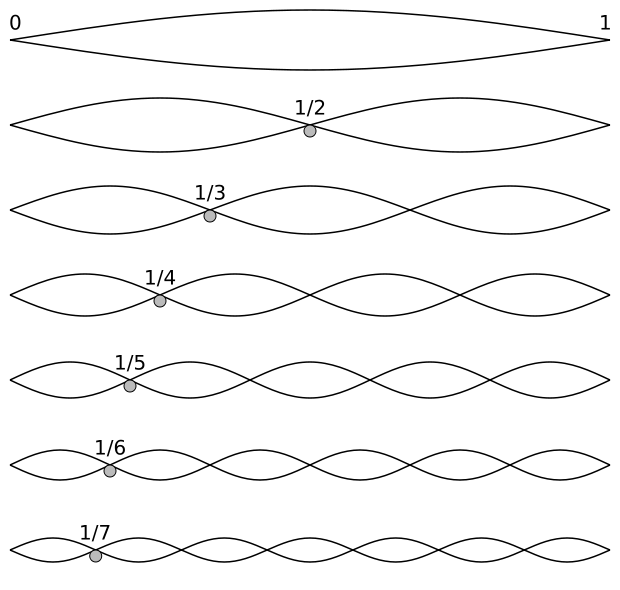
\includegraphics[scale=0.25]{Signale/Bilder/harmonische.png}
 \vspace{-6cm}
\end{wrapfigure}

\section*{Theorie- und Prüfungsfragen} 

\mucho{1}{TB608}
{Der Spitzenwert der häuslichen 230-V-Stromversorgung beträgt}%Frage
{163V}%A
{325V}%B
{460V}%C
{650V}%D
{B}%Lösung


\mucho{2}{TB610}
{Ein sinusförmiger Wechselstrom mit einer Amplitude ($I_max$) von 0,5A fließt durch einen Widerstand von 20$\Omega$. Wie hoch ist die aufgenommene Leistung?}%Frage
{0,5W}%A
{2,5W}%B
{5W}%C
{10W}%D
{B; $I = \dfrac{0,5A}{\sqrt{2}}= \dfrac{0,5A}{1,414} = 0,3536A; P=I^2\cdot R = (0,3536A)^2 \cdot 20 \Omega = 2,5W$}%Lösung

\mucho{3}{TB603}
{Wie groß ist der Spitzen-Spitzen-Wert des Signals in Abilldung \ref{sinus}?}%Frage
{12V}%A
{6V}%B
{8,5V}%C
{2V}%D
{A}%Lösung

\mucho{4}{TB604}
{Welche Frequenz hat das Signal in Abbildung \ref{sinus}?}%Frage
{833,3 kHz}%A
{83,3 kHz}%B
{8,3 MHz}%C
{83,3 MHz}%D
{B}%Lösung

\begin{figure}[H]
\centering
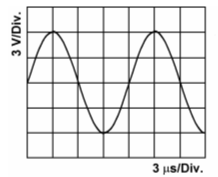
\includegraphics[scale=0.6]{Signale/Bilder/TB603.png}
\caption{Sinus-Signal}
\label{sinus}
\end{figure}

\mucho{5}{TB703}
{Was sind Harmonische?}%Frage
{Harmonische sind die ganzzahligen (1, 2, 3 ...) Vielfachen einer Frequenz.}%A
{Harmonische sind die ganzzahligen (1, 2, 3 ...) Teile einer Frequenz.}%B
{Harmonische sind die erzeugten Frequenzen oberhalb der ursprünglichen Frequenz.}%C
{Harmonische sind identisch mit den Oberwellen, wobei die Grundwelle keine Harmonische ist.}%D
{A}%Lösung

\mucho{6}{TB704}
{Die dritte Oberwelle einer Frequenz ist}%Frage
{die dritte Harmonische der Frequenz.
}%A
{die zweite Harmonische der Frequenz.}%B
{die zweite ungeradzahlige Harmonische der Frequenz.}%C
{die vierte Harmonische der Frequenz.}%D
{D}%Lösung

\mucho{7}{TB705}
{Welche Schwingungen sind in der folgenden Wechselspannung (Abbildung \ref{TB705})enthalten, wenn die Grundwelle 2 kHz beträgt?}%Frage
{4 kHz und 6 kHz}%A
{2 kHz und 6 kHz}%B
{4 kHz allein}%C
{2 kHz und 4 kHz}%D
{D}%Lösung

\begin{figure}[H]
\centering
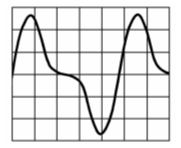
\includegraphics[scale=0.6]{Signale/Bilder/TB705.png}
\caption{Sägezahnschwingung durch Addition von Grundwelle und Harmonischer}
\label{TB705}
\end{figure}

\mucho{8}{TB706}
{ Welche Schwingungen sind in der folgenden Wechselspannung (Abbildung \ref{TB706}) enthalten, wenn die Grundwelle 2 kHz beträgt? }%Frage
{4 kHz und 6 kHz}%A
{2 kHz und 4 kHz}%B
{2 kHz und 6 kHz}%C
{4 kHz allein}%D
{C}%Lösung

\begin{figure}[H]
\centering
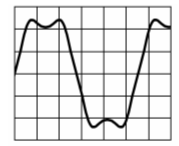
\includegraphics[scale=0.6]{Signale/Bilder/TB706.png}
\caption{Rechtecksignal aus der Summe von ungeradzahligen Harmonischen}
\label{TB706}
\end{figure}